\documentclass{article}

\usepackage{graphicx}
\usepackage{tikz}
\usepackage{tikzsymbols}
\usetikzlibrary{calc,patterns,shapes.geometric}
\pagestyle{empty}
\usepackage[margin=0pt]{geometry}
\geometry{papersize={14in,12in}}

\def\centerarc[#1](#2)(#3:#4:#5){\draw[#1] ($(#2)+({#5*cos(#3)},{#5*sin(#3)})$) arc (#3:#4:#5);}

\begin{document}
	\begin{figure}
		\centering
		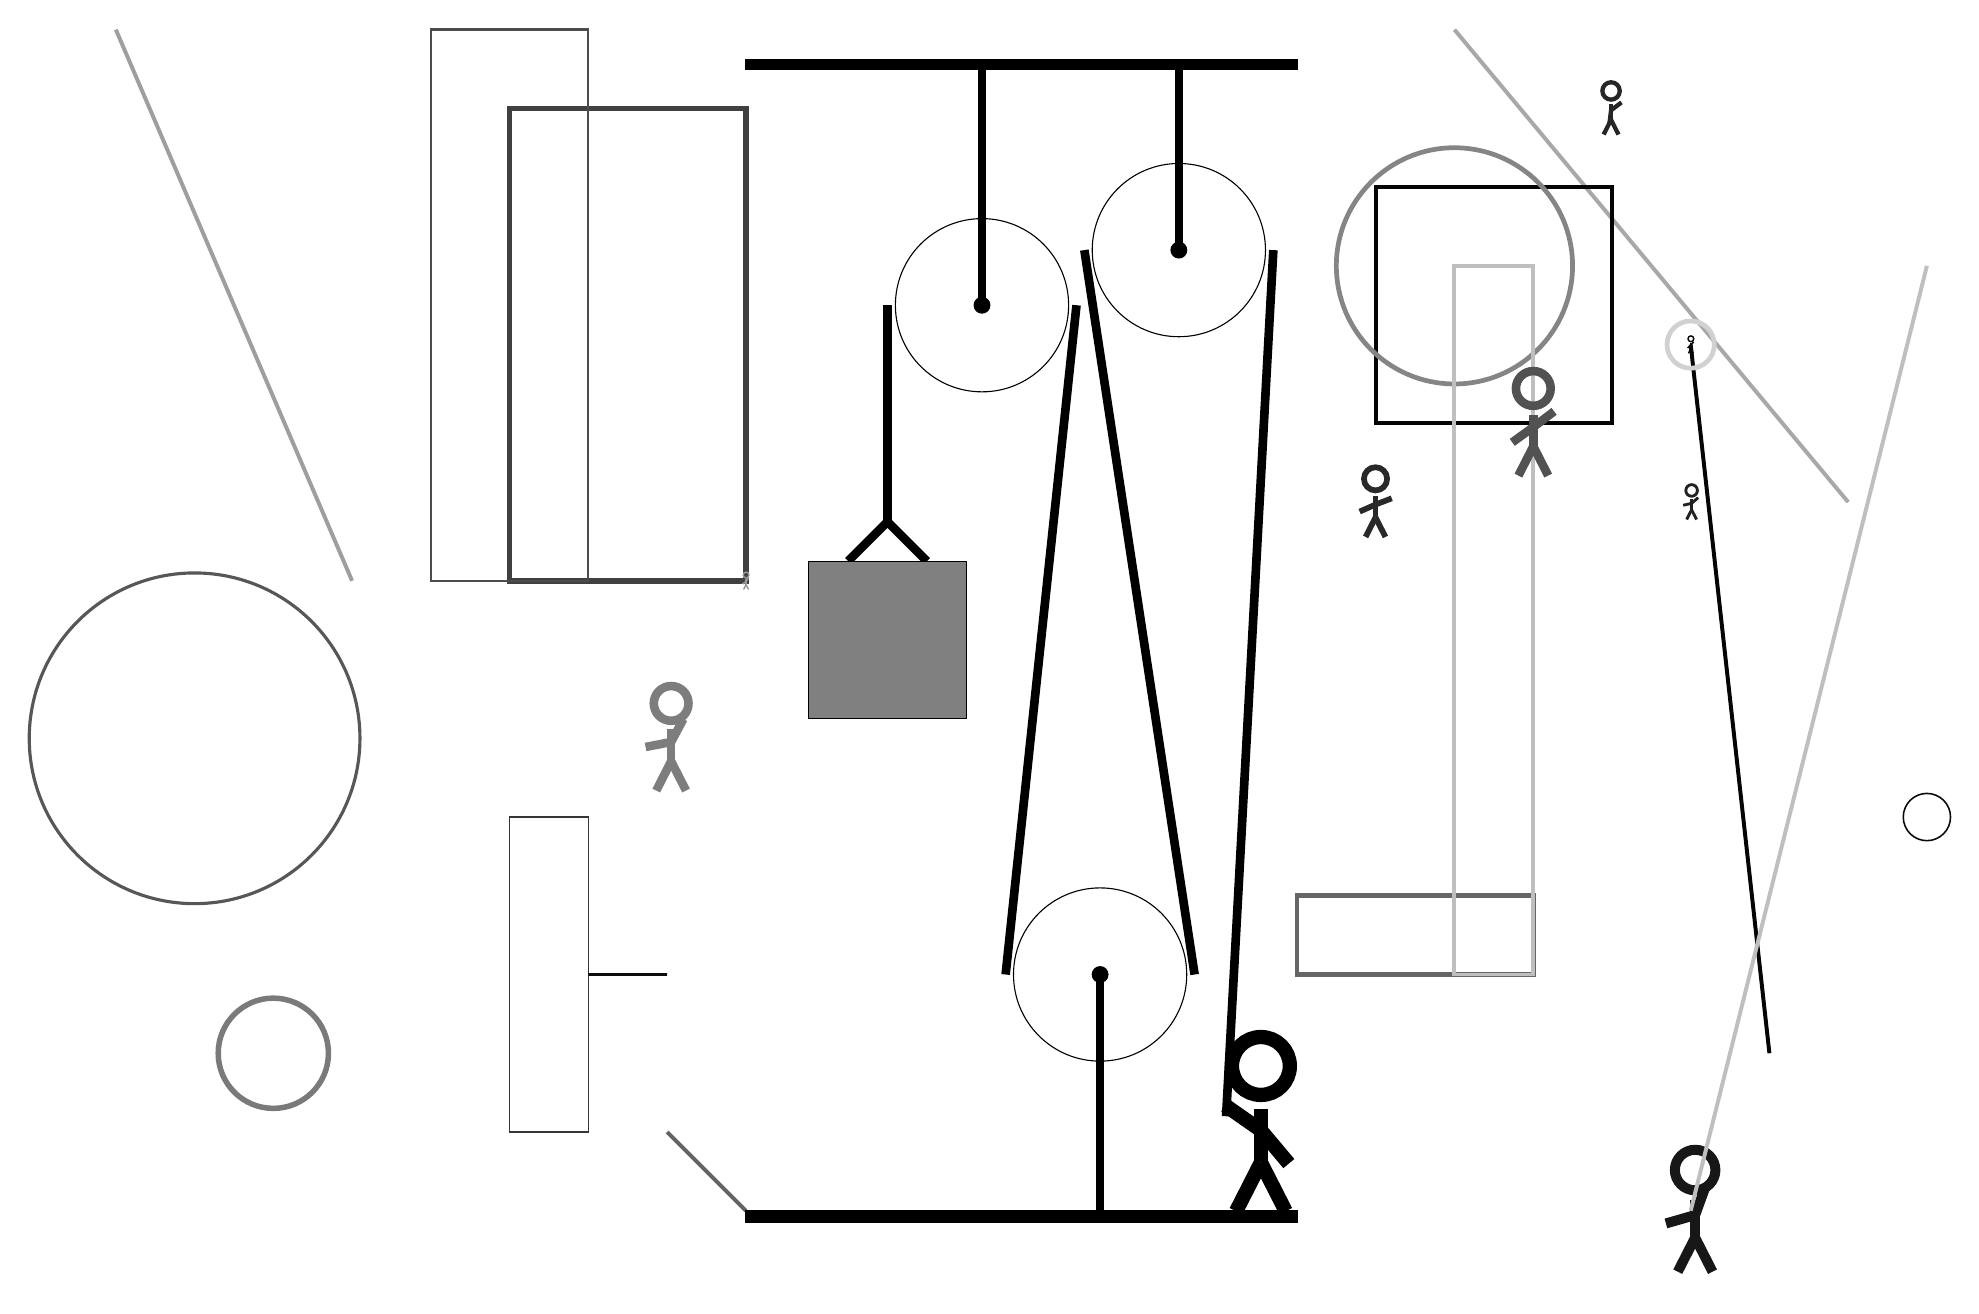
\begin{tikzpicture}
			%%%%% START %%%%%
			
			\draw[fill=black] (-2, 11.5) rectangle (5, 11.625);
			
			\draw (1, 8.5) circle (1.1);
			\draw[fill=black] (1, 8.5) circle (0.1);
			\draw[line width=1.1mm]  (1, 11.5) -- (1, 8.5);
			
			\draw[fill=white](2.5, 0.0) circle (1.1);
			\draw[fill=black] (2.5, 0.0) circle (0.1);
			\draw[line width=1.1mm]  (2.5, -3) -- (2.5, 0.0);
			
			\draw[fill=white](3.5, 9.2) circle (1.1);
			\draw[fill=black] (3.5, 9.2) circle (0.1);
			\draw[line width=1.1mm] (3.5, 11.5) -- (3.5, 9.2);
			
			\draw[line width=1.1mm] (-0.7, 5.25) -- (-0.2, 5.75) -- (0.3, 5.25);
			\draw[fill=black!50] (-1.2, 5.25) rectangle (0.8, 3.25);
			
			\draw[line width=0.5mm, color=black!34](7, 12) -- (12, 6);
			
			\draw[line width=0.7mm, color=black!75] (-2, 11) rectangle (-5, 5);
			\draw [line width=0.4mm, color=black!66](-9, 3) circle (2.1);
			\draw[line width=0.5mm, color=black!98](10, 8) -- (11, -1);
			\draw[line width=0.5mm, color=black!61](-2, -3) -- (-3, -2);
			\draw[line width=0.6mm, color=black!60] (5, 0) rectangle (8, 1);
			\draw [line width=0.2mm, color=black!96](13, 2) circle (0.3);
			
			\node[line width=0.3mm, color=black!40] at (-2, 5) {\Strichmaxerl[1][36][56]};
			\draw[line width=0.5mm, color=black!98] (6, 7) rectangle (9, 10);
			\draw[line width=0.2mm, color=black!79] (-4, -2) rectangle (-5, 2);
			\node[line width=0.5mm, color=black!84] at (6, 6) {\Strichmaxerl[4][24][21]};
			\draw [line width=0.6mm, color=black!18](10, 8) circle (0.3);
			\node[line width=0.2mm, color=black!87] at (10, 6) {\Strichmaxerl[2][13][41]};
			
			\draw [line width=0.6mm, color=black!48](7, 9) circle (1.5);
			\draw[line width=0.5mm, color=black!38](-7, 5) -- (-10, 12);
			\draw [line width=0.7mm, color=black!52](-8, -1) circle (0.7);
			
			\node[line width=0.6mm, color=black!91] at (10, -3) {\Strichmaxerl[7][16][70]};
			
			\draw[line width=0.5mm, color=black!25](10, -3) -- (13, 9);
			\draw[line width=0.3mm, color=black!70] (-4, 12) rectangle (-6, 5);
			\draw[line width=0.4mm, color=black!95] (-3, 0) rectangle (-4, 0);
			\draw[line width=0.5mm, color=black!25] (7, 9) rectangle (8, 0);
			\node[line width=0.4mm, color=black!85] at (9, 11) {\Strichmaxerl[3][83][37]};
			
			\node[line width=0.7mm, color=black!68] at (8, 7) {\Strichmaxerl[6][36][37]};
			\node[line width=0.2mm, color=black!97] at (10, 8) {\Strichmaxerl[1][39][51]};
			\node[line width=0.4mm, color=black!51] at (-3, 3) {\Strichmaxerl[6][11][62]};
			
			
			\draw[line width=1.1mm] (-0.2, 8.5) -- (-0.2, 5.75);
			\centerarc[line width=1.1mm](1, 8.5)(0:180:1.2000000000000002);
			\draw[line width=1.1mm](2.2, 8.5) -- (1.3, 0.0);
			\centerarc[line width=1.1mm](2.5, 0.0)(180:360:1.2000000000000002);
			\draw[line width=1.1mm](3.7, 0.0) -- (2.3, 9.2);
			\centerarc[line width=1.1mm](3.5, 9.2)(0:180:1.2000000000000002);
			\draw[line width=1.1mm](4.7, 9.2) -- (4.1, -1.8);
			
			\node at (4.5, -1.9) {\Strichmaxerl[10][-35][-50]};
			
			\draw[fill=black] (-2, -3) rectangle (5, -3.15);
			
			%%%%% END %%%%%
		\end{tikzpicture}
	\end{figure}	
\end{document}